% All contribution chapters should follow a similar structure, with a
% mini-introduction and overview at the beginning and a conclusion at the
% end bookmarking a structured presentation of the contribution. This can be
% largely based on your publications.

\chapter{Dimensional Analysis and Parameters}\label{chap:contrib2}

To validate the dimensions of the parameters in our simulations, we used two key parameters as reference points: the length of the bacteria (as a spatial reference) and the bacterial doubling time (as a temporal reference). The dimensions of the remaining parameters in this simulation, such as the diffusion coefficient, grid size, and reaction rates, were calculated relative to these two parameters.

\section{Spatial and Temporal Points of Reference}\label{sec:contrib2:theme1}

\subsection{Bacterial Length}\label{sec:contrib2:theme1:A}

In the context of a typical \textit{Bacillus subtilis} cell, which measures approximately 6 µm in length, we defined the reproductive length as a random variable with a uniform distribution between 12 and 12.1 µm. Consequently, the maximum length that a bacterial cell can reach is approximately 12 µm just before binary fission, while the minimum length is about 6 µm immediately after binary fission.

\subsection{Bacterial Doubling Time}\label{sec:contrib2:theme1:B}

The growth rate per simulation time step is defined as a dimensionless random variable uniformly distributed between 1.002 and 1.003. The range of this random variable was intentionally chosen to ensure that the physics engine library can accurately compute the volume exclusion forces at each simulation time step without any unresolved overlaps. A higher growth rate would lead to rapid cell growth, causing excessive overlap in volume between the bodies of the bacteria. If the overlap is too large, it may not be fully resolved by the physics engine within a single simulation time step. The random fluctuation in the growth rate causes the size of bacteria, on average, to increase by a factor of 1.0025 at each time step.

While it might have been possible to calculate the exact doubling time analytically by assuming a constant growth rate, constant reproductive length across the population, and assuming that bacterial bodies are perfectly rectangular (as opposed to rods with rounded ends), we chose to estimate the doubling time through numerical simulations. This numerical methodology was chosen as a practical approach to account for the stochastic nature of the bacteria's growth rate and reproductive cycle, as well as the nuance that the length of the bacteria does not exactly represent the distance from one rounded end to the other rounded end of the bacteria.

\begin{figure}[h]
    \centering
    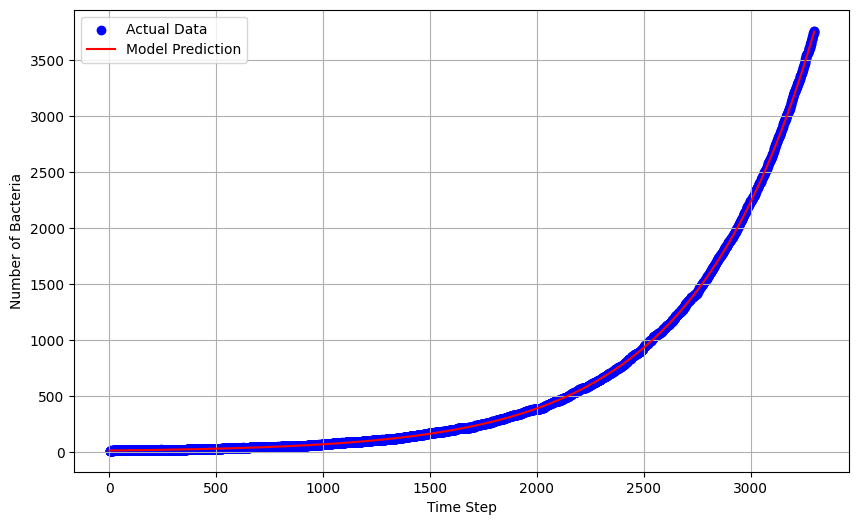
\includegraphics[width=1\textwidth]{Exponential_growth}
    \caption{\footnotesize \textbf{Bacteria cell count over simulation time steps.} The total number of bacteria in the simulation after each time step is shown in blue. The fitted model for exponential growth is shown in red.}

\end{figure}

To calculate the doubling time, we allowed the bacteria to grow and reproduce until the population reached approximately 3700 bacteria, similar to the growth and reproduction progression depicted in Figure 3.3. We recorded the number of bacteria at each time step of the simulation. Figure 4.1 illustrates the cumulative bacterial count during a growth simulation. The bacterial doubling time was determined by fitting a non-linear regression model to the data points obtained from simulations. The exponential growth equation \(y = b \cdot e^{mt}\) is used as a model, where \(y\) represents the cell count at the discrete time step \(t\), \(b\) represents the initial cell count, and \(m\) represents the growth rate.

In the fitted regression model, the parameters \(b\) and \(m\) were estimated to be approximately 11.74 bacteria and 0.00175, respectively. The coefficient of determination $(R^2)$ for this model is approximately 0.9997.

The estimated parameter \(m\) can be used to calculate the doubling time \(\tau\) using the following equation:


\[
    \tau=\frac{{\ln(2)}}{m} 
\]

which results in a doubling time of $\approx$ 396 simulation time steps.


Given that the actual doubling time of \textit{Bacillus subtilis} in optimal conditions is around 30 minutes, we can use the above estimate to set one simulation time step to represent 5 seconds. Taking this into consideration, the calculated doubling time for the simulated bacteria is 33 minutes.





\section{Numerical Simulation of the Diffusion Equation}\label{sec:contrib2:theme2}

The diffusion equation is a partial differential equation that describes the behavior of a substance as it spreads out over time due to random motion. It serves as a fundamental model for understanding heat distribution, particle dispersion, and other processes characterized by the flow from regions of higher concentration to regions of lower concentration. The standard form of the diffusion equation in two dimensions is:

\[
\frac{\partial u}{\partial t} = D \left( \frac{\partial^2 u}{\partial x^2} + \frac{\partial^2 u}{\partial y^2} \right),
\]

where $u$ represents the concentration of the diffusing substance at a given point, $D$ is the diffusion coefficient, and $t$, $x$, and $y$ are the time and spatial variables, respectively. {\footnotesize\cite{caltech}}

To numerically simulate the diffusion equation, we apply the finite difference method, which is a well-established numerical technique for solving partial differential equations. This involves discretizing the spatial domain into a grid and approximating the continuous derivatives with respect to time and space by using the differences between grid point values. We construct a matrix representation of the diffusion field \(u_{n+1}[i,j]\), which represents the concentration of substance \(u\) at each grid position \([i,j]\) and at each time step \(n+1\).

The concentration \(u\) is updated iteratively for each grid position based on the previous time step \(n\) and the influence of its neighboring grid points. This update is governed by the discrete diffusion equation:

\[
u_{n+1}[i][j] = u_{n}[i][j] + \gamma  \left( u_{n}[i+1][j] + u_{n}[i][j+1] + u_{n}[i-1][j] + u_{n}[i][j-1] - 4  u_{n}[i][j] \right)
\]

where \(\gamma\) is a constant given by 

\[ \gamma = D \frac{{\Delta t}}{{(\Delta x)^2}},  \]

with \(D\) being the diffusion coefficient of $u$, \(\Delta t\) representing the time step increment, and \(\Delta x\) signifying the spatial step size or the grid resolution. {\footnotesize\cite{gitconnectedSolvingHeat}\cite{unimuenster}}

To ensure computational stability for this numerical method, it is crucial to satisfy the following condition, which requires the time step \(\Delta t\) to be sufficiently small:

\[\frac{{\Delta t}}{{(\Delta x)^2}} \leq \frac{1}{{4D}}.\]

Fulfilling this criterion ensures the convergence of the solution and helps to avoid numerical oscillations. {\footnotesize\cite{gitconnectedSolvingHeat}\cite{unimuenster}}

For a rough estimate of the diffusion constant \(D\) of signaling molecules in our simulation, we can consider the order of magnitude to be similar to that of glucose diffusing in water, which is roughly 100 \(\mu m^2/s\) {\footnotesize\cite{Bashkatov2003}}. With a specified grid resolution in which each element has an area of 10 \(\mu m\) by 10 \(\mu m\), the stability condition can be used to calculate the maximum allowable time step \(\Delta t\) to solve the diffusion equation, yielding \(t \leq 0.25\) s.

Since the time step for bacterial growth is 5 seconds (as calculated in section 4.1.2), we need to perform the diffusion numerical iterations more frequently than the time step in which the bacteria are growing. This means that for each time-step that the bacteria use to grow, the diffusion equation undergoes 20 time-steps to update the concentration of the extracellular signaling molecules.


\section{Regulatory gene circuit}\label{sec:contrib2:theme2}


The agent-based model simulates the evolution of cytoplasmic concentrations of regulatory proteins by solving the system of differential equations described in Section 2.4.3. The Euler method was used to solve the equations using a time step of 1 minute. This 1-minute time step was determined through a trial-and-error process aimed at finding the largest possible time step that maintains computational efficiency without compromising the stability of the numerical simulation. During the trial-and-error process, we utilized the three-dimensional phase space to track the trajectories of SinR, SinI, and SlrR concentrations over time. The code for visualizing the solutions in phase space is provided in section 7.3.

The magnitude and dimensions of the parameters used to simulate this system of equations are presented in Table 4.1. These parameters are based on the typical rates and thresholds observed in biological systems. However, they are still rough approximations of the exact real values for the case of \textit{B. subtilis}. Most of the parameters shown in Table 4.1 were chosen with reference to the models and estimations presented in ({\footnotesize\cite{simon}\cite{Voigt2005}\cite{Newman2013}\cite{Chen2023}\cite{Pedreira2021}\cite{Hallinan2010}}).

Two parameters, \(K_A\) and \(K_R\), were defined as uniformly distributed variables across the population to introduce stochasticity into the system of differential equations. The reason for introducing this slight stochasticity into these two parameters is that we do not expect real bacteria to have identical effective reaction rates with every other bacterium. In reality, we assumed that the effective reaction rates vary across the population due to diverse cytoplasmic conditions unique to each bacterium, including other inhibitors and activators not accounted for in this model, such as SlrA and AbrB. The parameters were fine-tuned by observing the behavior of the solution trajectories in phase space and ensuring that they replicated the expected switch-like behavior previously documented in the literature. In any case, the parameters were kept within typical values for biological systems.

  \begin{table}
    \centering
    \caption{\footnotesize Parameters for SinR-SlrR-SinI gene regulatory network}
    \label{table:parameters}
    \begin{tabular}{|c|c|c|}
      \hline
      Parameter & Value & Units  \\
      \hline
      \(P_3\) & 1.5 & nM/minute \\
      \(P_1\) & 1.5 & nM/minute \\
      \(P_L\) & 1.25 & nM/minute \\
      
      \(D_R\) & 1.4 \(\times 10^{-2}\) & 1/minute  \\   
      \(D_I\) & 1.4 \(\times 10^{-2}\) & 1/minute  \\
      \(D_L\) & 1.4 \(\times 10^{-2}\) & 1/minute  \\ 
      \(K_{on(RL)}\) & 1 \(\times 10^{-3}\) & 1/(minute\(\cdot\)nM)  \\
      \(K_{on(RI)}\) & 1 \(\times 10^{-3}\) & 1/(minute\(\cdot\)nM)  \\ 

      
      \(K_A\) & \( \sim U(47.5, 52.5)\) & nM  \\
      \(K_R\) & \( \sim U(52.5, 57.5)\) & nM \\

      

      \(n_A\) & 4 & -  \\
      
      \(n_R\) & 4 & -  \\
    
      \hline
    \end{tabular}
  \end{table}
  \section{Secretion of Signaling Molecules}\label{sec:contrib2:theme2}
  Our understanding of the exact rates at which ComX and surfactin are produced and degraded during the various stages of \textit{B. subtilis} biofilm development is still incomplete. Similarly, the exact concentrations of surfactin, ComX, and SinR that induce a phenotype transition are not completely clear. To address this, we have designed our agent-based model to represent the concentrations of ComX and surfactin in arbitrary units (AU). Future studies could then adjust these dimensionless concentrations using experimental parameters obtained from real-world data.
  
  We have designed the simulation so that every 0.25 seconds (the same time step as for solving the diffusion equation), every single bacterium secretes a small fixed amount of ComX, regardless of the cell's specific phenotype. In addition to the ComX that every bacterium secretes, bacteria belonging to the surfactin-producing phenotype also secrete an additional fixed amount of surfactin at the same time step. This means that surfactin producers secrete two signaling molecules: ComX and surfactin. Non-surfactin producers will only produce ComX. The reason why every bacterium in our simulation produces ComX is that we assumed that the \textit{comX} gene is constitutively expressed.

  Given that the number of surfactin producers is significantly smaller than the number of ComX producers, we set the surfactin production to be ten times that of the ComX production. This makes it easier to visualize and compare the concentration of both substances during the simulation.

  \section{Conclusion}

  Having established the mathematical methods and the arguments for the parameters and assumptions used in the simulation, we can now proceed to the simulation results. The results will be presented in the following chapter.
    
  
  
